%%%%%%%%%%%%%%%%%%%%%%%%%%%%%%%%%%%%%%%%%%%%%%%%%%%%%%%%%%%%%%%%%%%%%%%%%%%%
% 26/05/2010
% edited by Bill Lampos
%
% Feel free to use (copy) the structure (latex formatting source code)
% but not the content of this document.
%
%%%%%%%%%%%%%%%%%%%%%%%%%%%%%%%%%%%%%%%%%%%%%%%%%%%%%%%%%%%%%%%%%%%%%%%%%%%%%
\documentclass[mathserif,compress,red]{beamer}
\mode<presentation>

\usetheme{Warsaw}
% other themes: AnnArbor, Antibes, Bergen, Berkeley, Berlin, Boadilla, boxes, CambridgeUS, Copenhagen, Darmstadt, default, Dresden, Frankfurt, Goettingen,
% Hannover, Ilmenau, JuanLesPins, Luebeck, Madrid, Maloe, Marburg, Montpellier, PaloAlto, Pittsburg, Rochester, Singapore, Szeged, classic

\usecolortheme{default}
% color themes: albatross, beaver, beetle, crane, default, dolphin, dov, fly, lily, orchid, rose, seagull, seahorse, sidebartab, structure, whale, wolverine

%\usefonttheme{serif}
% font themes: default, professionalfonts, serif, structurebold, structureitalicserif, structuresmallcapsserif

% pdf is displayed in full screen mode automatically
%\hypersetup{pdfpagemode=FullScreen}

% define your own colours:
\definecolor{Red}{rgb}{1,0,0}
\definecolor{Blue}{rgb}{0,0,1}
\definecolor{Green}{rgb}{0,1,0}
\definecolor{magenta}{rgb}{1,0,.6}
\definecolor{lightblue}{rgb}{0,.5,1}
\definecolor{lightpurple}{rgb}{.6,.4,1}
\definecolor{gold}{rgb}{.6,.5,0}
\definecolor{orange}{rgb}{1,0.4,0}
\definecolor{hotpink}{rgb}{1,0,0.5}
\definecolor{newcolor2}{rgb}{.5,.3,.5}
\definecolor{newcolor}{rgb}{0,.3,1}
\definecolor{newcolor3}{rgb}{1,0,.35}
\definecolor{darkgreen1}{rgb}{0, .35, 0}
\definecolor{darkgreen}{rgb}{0, .6, 0}
\definecolor{darkred}{rgb}{.75,0,0}

\xdefinecolor{olive}{cmyk}{0.64,0,0.95,0.4}
\xdefinecolor{purpleish}{cmyk}{0.75,0.75,0,0}

% \usepackage{beamerinnertheme_______}
% inner themes include circles, default, inmargin, rectangles, rounded

%\usepackage{beamerouterthemesmoothbars}
% outer themes include default, infolines, miniframes, shadow, sidebar, smoothbars, smoothtree, split, tree

\useoutertheme[subsection=false]{smoothbars}

% to have the same footer on all slides
%\setbeamertemplate{footline}[text line]{xxx xxx xxx}
%\setbeamertemplate{footline}[text line]{} % or empty footer

% include packages
\usepackage{etex}
\usepackage{subfigure}
\usepackage{multicol}
\usepackage{amsmath}
\usepackage{epsfig}
\usepackage{graphicx}
\usepackage[all,knot]{xy}
\xyoption{arc}
\usepackage{url}
\usepackage{multimedia}
\usepackage{hyperref}
\usepackage{setspace}
\usepackage{verbatim}
\usepackage{enumerate}

\title{VFH$^{+}$ : Vector Field Histogram Plus}
\subtitle{Enhanced Obstacle Avoidance Algorithm}
\author{John Liu}
\institute{{\tiny Advisor:}\\ \vspace{.10cm}Professor Ying-Jeng Wu}
\date{\scriptsize Measurement Laboratory, National Yunlin University of Science \& Technology\\ \vspace{.10cm}March 12, 2014}

\begin{document}

\frame{
	\titlepage
}

\section{Outline}
\frame{\tableofcontents}

\section{Common Obstacle Avoidance Overview}
\subsection{Artificial Potential Field}
\frame{\frametitle{Artificial Potential Field}
Artificial Potential Field creates a virtual force field which attracts the robot toward the target, and retracts it away from the obstacle.
\begin{columns}
	\begin{column}{5cm}
	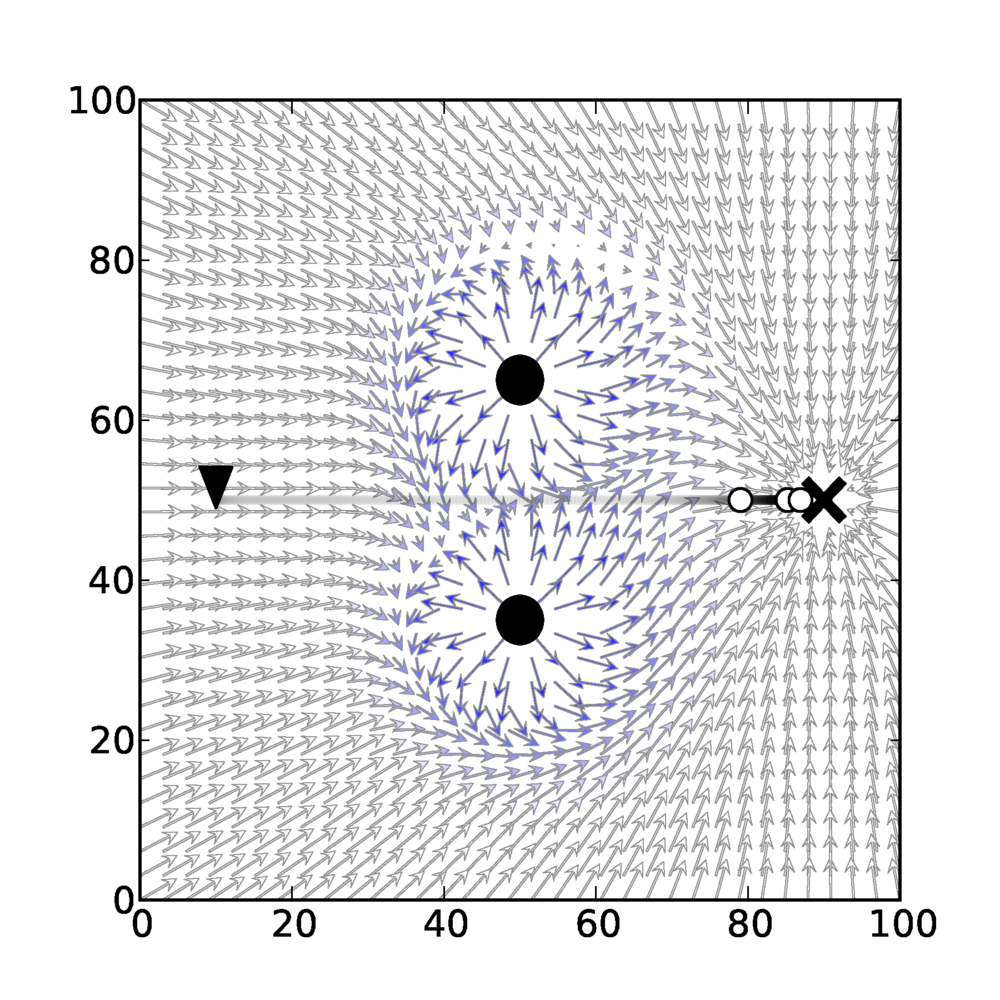
\includegraphics[scale=.18]{figures/APF.png}
	\end{column}
	\begin{column}{5cm}
	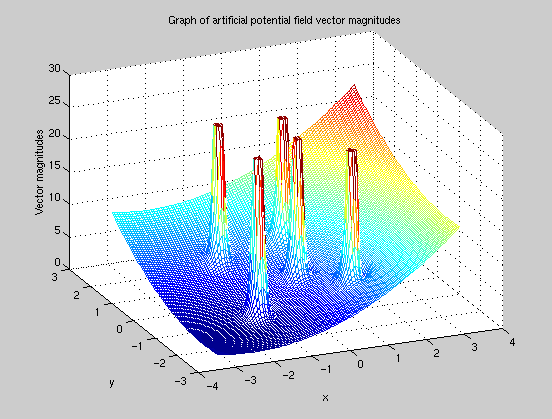
\includegraphics[scale=.25]{figures/demo_apf.png}
	\end{column}
\end{columns}
}

\frame{\frametitle{Artificial Potential Field}
\begin{itemize}
	\item Advantages:
	\begin{itemize}
		\item Global path planning
		\item Efficient Calculation
		\item Easily adapt to the data acquired by LiDAR
	\end{itemize}
	\vspace{0.25cm}
	\item Disadvantages:
	\begin{itemize}
		\item Ignore the kinematic and dynamic constraints
		\item Ignore robot's geometry
	\end{itemize}
\end{itemize}
}

\subsection{Vector Field Histogram}
\frame{\frametitle{Vector Field Histogram (VFH)}
VFH generates a polar histogram of the environment around the robot, identifies wide-enough spaces and calculates corresponding steering direction.
\begin{figure}
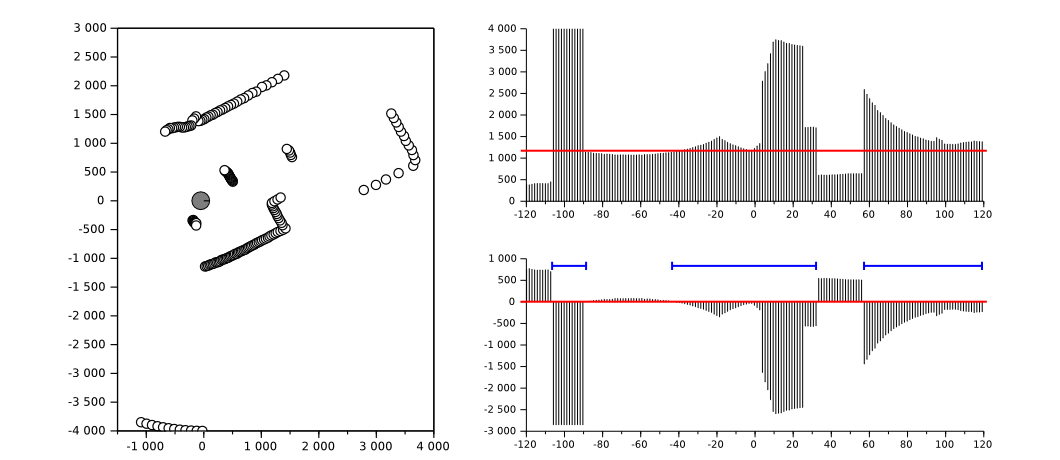
\includegraphics[scale=.37]{figures/VFH.png}
\end{figure}
}

\frame{\frametitle{Vector Field Histogram (VFH)}
A cost function $G$ is then applied to every candidate directions, and the direction which generates the smallest value is then selected:
\begin{equation*}
G = u_{1} \cdot \alpha + u_{2} \cdot \beta + u_{3} \cdot \gamma
\end{equation*}
where
\begin{align*}
	\alpha &= \text{difference between target and candidate direction} \\
	\beta &= \text{difference between current direction and candidate direction} \\
	\gamma &= \text{difference between the previously selected direction and candidate direction}
\end{align*}
$u_{1}$, $u_{2}$ and $u_{3}$ are weighting constants
}

\frame{\frametitle{Vector Field Histogram (VFH)}
\begin{itemize}
	\item Advantages:
	\begin{itemize}
		\item Easily adapt to the data acquired by LiDAR
		\item Efficient Calculation
		\item Adjustable characteristic
	\end{itemize}
	\vspace{0.25cm}
	\item Disadvantages:
	\begin{itemize}
		\item Ignore the kinematic and dynamic constraints
		\item Ignore robot's geometry
		\item \textbf{Direction depends on free-spaces}
	\end{itemize}
\end{itemize}
}

\subsection{Curvature Velocity Method}
\frame{\frametitle{Curvature Velocity Method (CVM)}
CVM takes robot's kinematic constraints into account, assumes it only travels along circular trajectories with curvature $c =  \omega / \nu$,
where $\omega$ is the rotational velocity and $\nu$ is the translational velocity with limits.
\begin{figure}
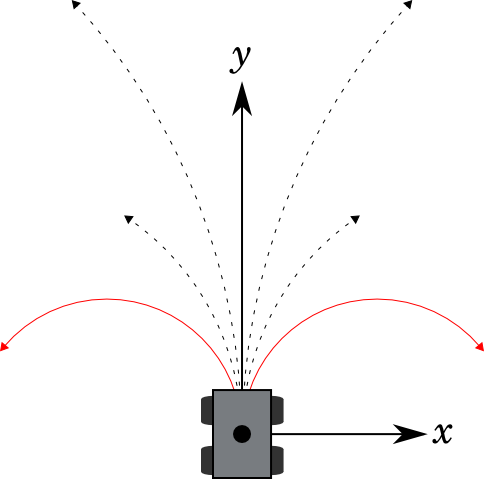
\includegraphics[scale=.35]{figures/CVM1.png}
\end{figure}
}

\frame{\frametitle{Curvature Velocity Method (CVM)}
The travelled distance $d_{v}$ of each obstacle can be calculated, and selected by a cost function.
For real-time implementation, There are some simplifications:
\begin{columns}[t]
\begin{column}{5cm}
	\begin{itemize}
		\item Obstacles are circular shaped
		\item $d_{v}$ between each $c_{min}$ and $c_{max}$ of an obstacle is divided onto few intervals with constant value
	\end{itemize}
\end{column}
\begin{column}{5cm}
	\begin{figure}
	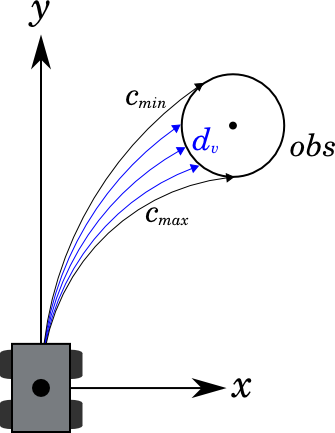
\includegraphics[scale=.35]{figures/CVM2.png}
	\end{figure}
\end{column}
\end{columns}
}

\frame{\frametitle{Curvature Velocity Method (CVM)}
The final decision of new $\omega$ and $\nu$ is made by an object function, which resembles the cost function of previous method:
\begin{equation*}
f(\omega,\nu) = u_{1} \cdot speed(\nu) + u_{2} \cdot dist(\omega,\nu) + u_{3} \cdot head(\omega)
\end{equation*}
where
\begin{align*}
speed(\nu) &= \nu / \nu_{max} \\
dist(\omega,\nu) &= d_{v} / d_{max} \\
head(\omega) &= 1 - |\theta_{target} - \omega \cdot T_{c} | / \pi \\
\end{align*}
The velocities which generate the largest value will be chosen!
}

\frame{\frametitle{Curvature Velocity Method (CVM)}
\begin{itemize}
	\item Advantages:
	\begin{itemize}
		\item Kinematic and dynamic constraints
		\item Robot's geometry constraint
		\item Adjustable characteristic
	\end{itemize}
	\vspace{0.25cm}
	\item Disadvantages:
	\begin{itemize}
		\item Simplified circular obstacle
		\item \textbf{Velocity sensors are required}
	\end{itemize}
\end{itemize}
}

\subsection{Dynamic Window Approaches}
\frame{\frametitle{Dynamic Window Approach (DW)}
DW also assumes the robot only travelled in circular path with rotational velocity $\omega$ and translational velocity $\nu$.
The sensed environment is then transformed into \textbf{velocity space}.
\begin{figure}
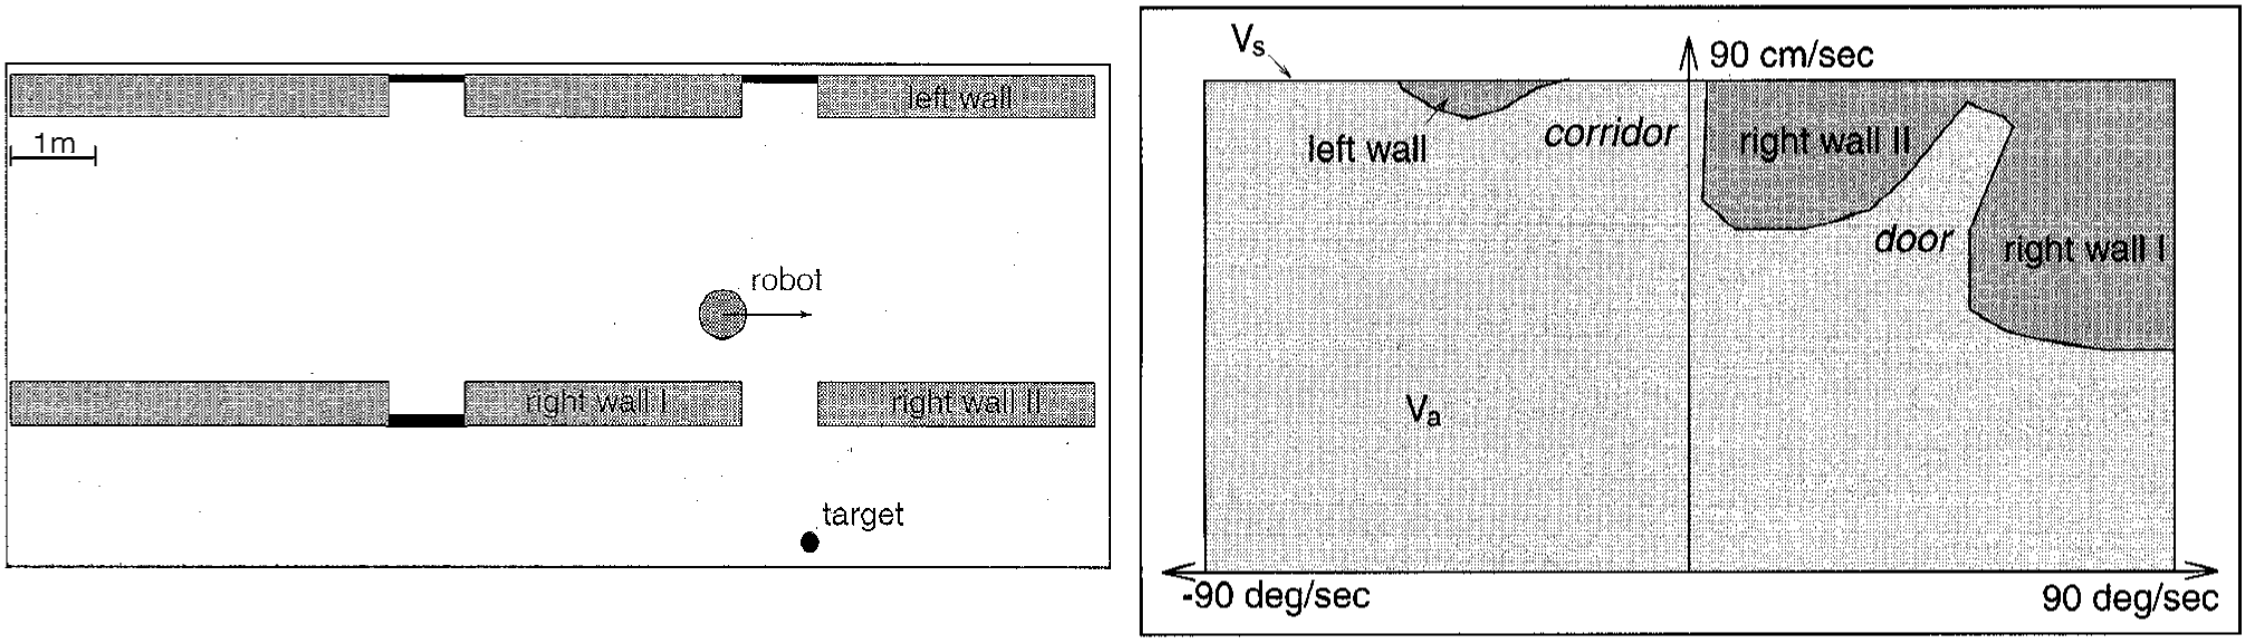
\includegraphics[scale=.17]{figures/DW1.png}
\end{figure}
}

\frame{\frametitle{Dynamic Window Approach (DW)}
In velocity space, a \emph{dynamic window} is constructed according to its dynamic constraints and current velocities.
Again, an object function is used to choose the optimized velocities.
\begin{figure}
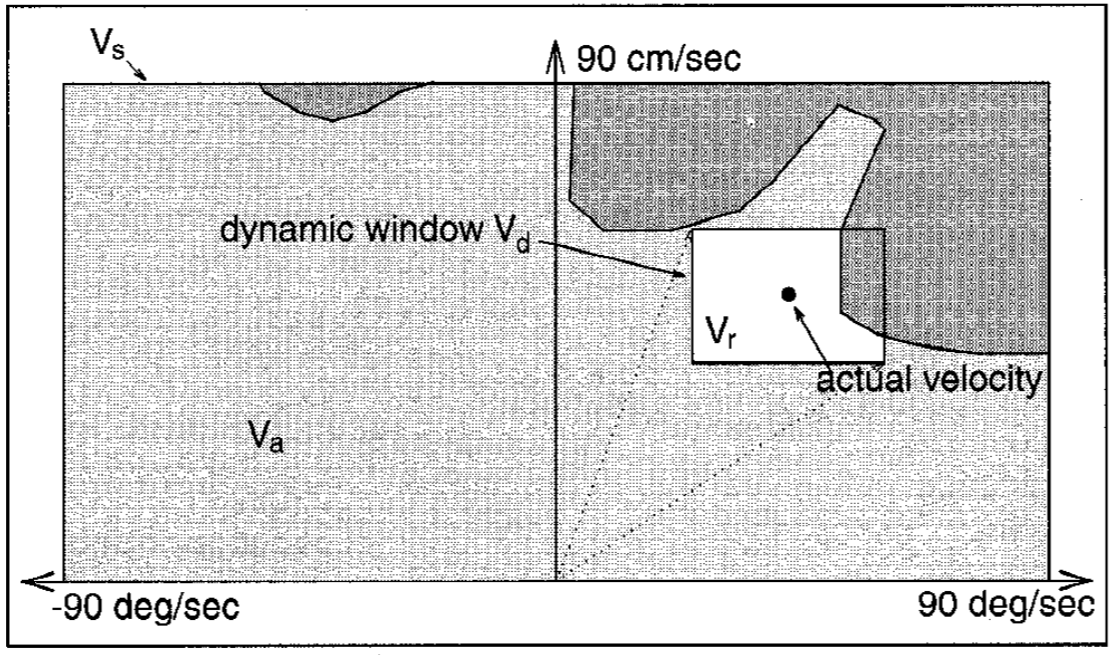
\includegraphics[scale=.25]{figures/DW2.png}
\end{figure}
}

\frame{\frametitle{Dynamic Window Approach (DW)}
\begin{itemize}
	\item Advantages:
	\begin{itemize}
		\item Kinematic and dynamic constraints
		\item Robot's geometry constraint
		\item Adjustable characteristic
	\end{itemize}
	\vspace{0.25cm}
	\item Disadvantages:
	\begin{itemize}
		\item Complexity
		\item \textbf{Velocity sensors are required}
	\end{itemize}
\end{itemize}
}

\section{Vector Field Histogram Plus}
\subsection{Introduction}
\frame{\frametitle{Vector Field Histogram Plus (VFH$^{+}$) - Introduction}
VFH$^{+}$ algorithm is an enhanced version of original VFH which offers several improvements:
\begin{enumerate}
	\vspace{0.25cm}
	\item Kinematic constraints
	\vspace{0.25cm}
	\item Robot's geometry constraints
	\vspace{0.25cm}
	\item \textbf{Direction no longer depends on spaces}
\end{enumerate}
}

\frame{\frametitle{VFH$^{+}$ - Four-Stage Process}
The VFH$^{+}$ employs a four-stage data reduction process in order to compute the new direction of motion:
\begin{enumerate}
	\vspace{0.25cm}
	\item Primary Polar Histogram
	\vspace{0.25cm}
	\item Binary Polar Histogram
	\vspace{0.25cm}
	\item Masked Polar Histogram
	\vspace{0.25cm}
	\item Selection of Steering Direcion
	\vspace{0.25cm}
\end{enumerate}
}

\frame{\frametitle{VFH$^{+}$ - with Laser Range Finder}
However, some modification is required in order to implement VFH$^{+}$ with laser range finder, therefore the process become:
\begin{enumerate}
	\vspace{0.25cm}
	\item Primary Polar Histogram
	\vspace{0.25cm}
	\item Free Spaces
	\vspace{0.25cm}
	\item Blocked Directions
	\vspace{0.25cm}
	\item Selection of Steering Direction
	\vspace{0.25cm}
\end{enumerate}
}

\subsection{Algorithm of Steering Direction}
\frame{\frametitle{1: Primary Polar Histogram}
A polar histogram $P_i$ of corresponding measured distance and angle $d_i$ can be generated with following formula:
\begin{equation*}
	P_i = a + b \cdot d_i
\end{equation*}
\begin{figure}
	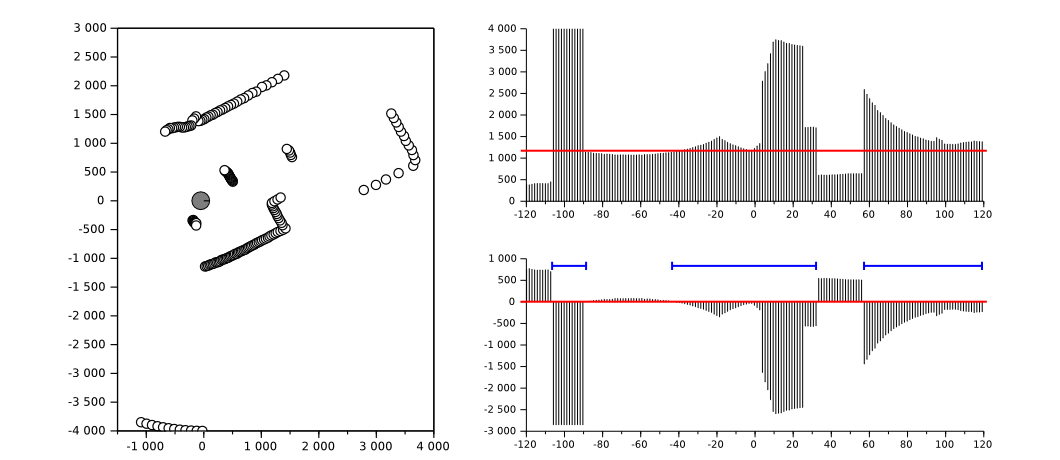
\includegraphics[scale=.33]{figures/VFH.png}
\end{figure}
}

\frame{\frametitle{2: Free Spaces - Hysteresis Filter}
VFH$^+$ uses two thresholds $\tau_{max}$ and $\tau_{min}$ instead of single threshold $\tau$ in VFH
to overcome the oscillation motion in environments with several narrow opennings:
\[
	P'_i = 
	\begin{cases}
		P_i	& \textrm{if } P_i \geq \tau_{max} \\
		0	& \textrm{if } P_i \leq \tau_{min} \\
		P_{i-1}	& \textrm{otherwise}
	\end{cases}
\]
\begin{figure}
	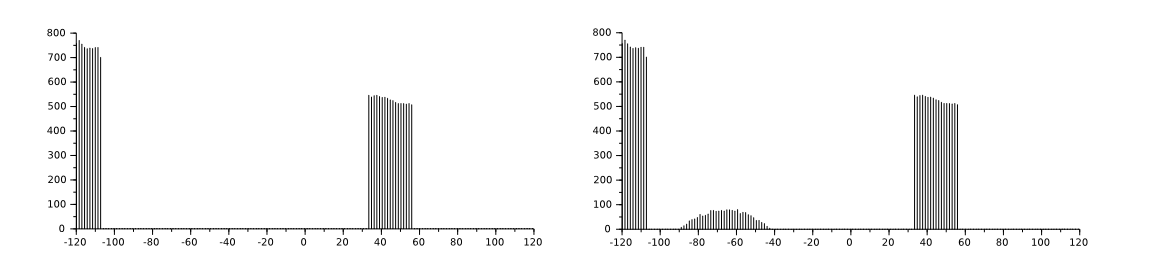
\includegraphics[scale=.35]{figures/HysteresisFilter2.png}
\end{figure}
}

\frame{\frametitle{2: Free Spaces - Boundary}
Each valley of filtered polar histogram $P'_i$ indicates safe directions for the robot, namely $V_j$.
\begin{columns}[c]
	\begin{column}{5cm}
		The boundaries of each $V_j$ are defined by two angle:
		\begin{equation*}
			V_j = (\theta_j^r,\theta_j^l)
		\end{equation*}
	\end{column}
	\begin{column}{5cm}
		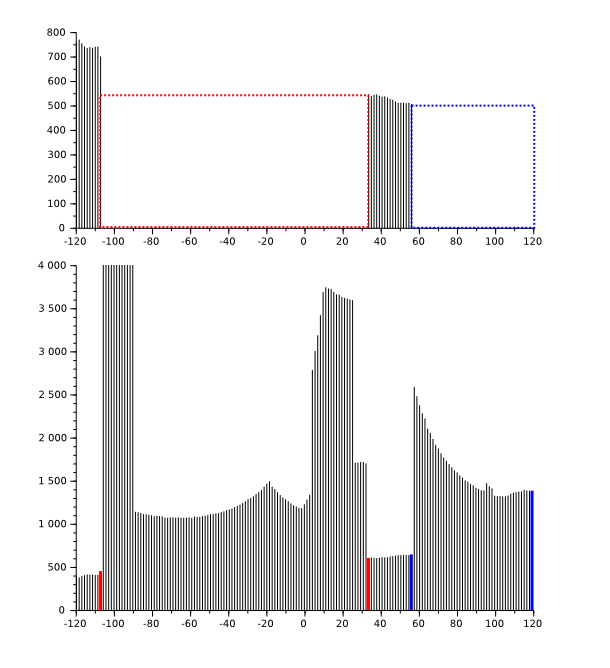
\includegraphics[scale=.32]{figures/FreeSpacesBoundaries.png}
	\end{column}
	
\end{columns}
}

\frame{\frametitle{2: Free Spaces - Robot's Geometry}
With geometry constraints, new boundaries $V_j' = (\theta_j^r{}',\theta_j^l{}')$ of each $V_j$ are calculated:
\begin{columns}[t]
	\begin{column}{5cm}
		\begin{align*}
			\theta_j^r{}'	&= \theta_j^r + \gamma^r \\
					&= \theta_j^r + \arcsin(w_s / d^r)\\
			\intertext{and}
			\theta_j^l{}'	&= \theta_j^l - \gamma^l \\
					&= \theta_j^l - \arcsin(w_s / d^l)\\
			\intertext{where $d^r$ and $d^l$ are corresponding measured distances.}
		\end{align*}
	\end{column}
	\begin{column}{5cm}
		\begin{figure}
		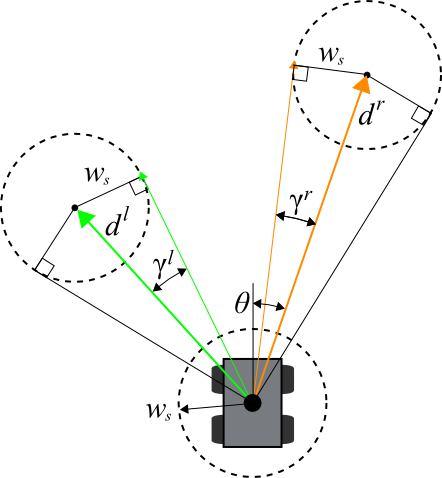
\includegraphics[scale=.4]{figures/Width.png}
		\end{figure}
	\end{column}
\end{columns}
}

\frame{\frametitle{2: Free Spaces - Overlapped}
The $V_j'$ with overlapped boundaries where $\theta_j^r{}' \geq \theta_j^l{}'$ are abandoned, since they are considered too narrow to pass through.
\begin{figure}
	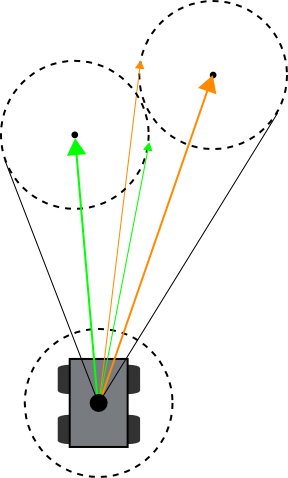
\includegraphics[scale=.4]{figures/WidthOverlapped.png}
\end{figure}
}

\frame{\frametitle{3: Blocked Directions}
VFH$^+$ also assumes circular trajectories of robot's motion.
However, this assumpation only used to determine the limitation of steering angles $\varphi_r$ and $\varphi_l$:
\begin{figure}
	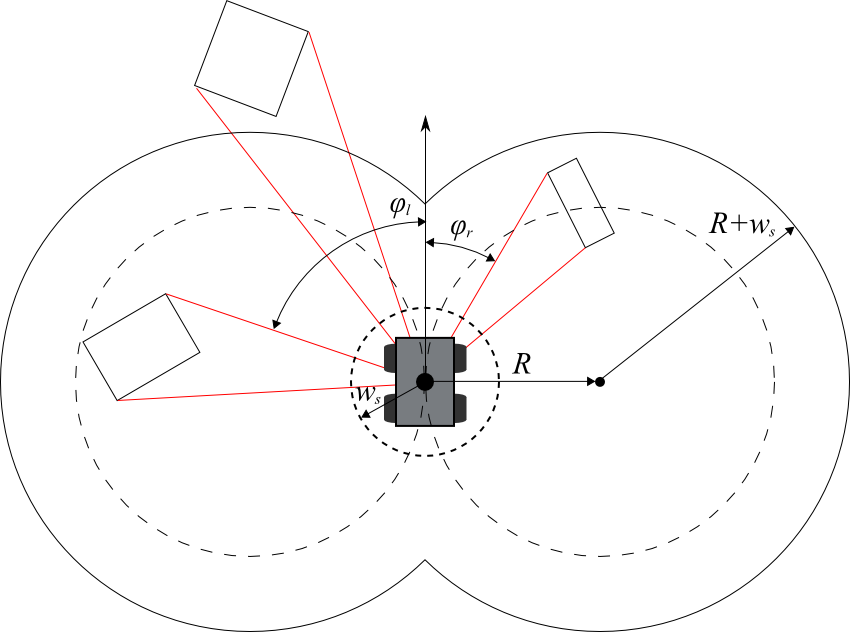
\includegraphics[scale=.3]{figures/Blocked.png}
\end{figure}
}

\frame{\frametitle{3. Blocked Directions - Detection Histogram}
In order to calculate $\varphi_r$ and $\varphi_l$, the detection histogram $D_i$ is generated first:
\begin{equation*}
	D_i = |R\sin\theta_i| + \sqrt{R^2\sin^2\theta_i + w_s^2 + 2Rw_s}
\end{equation*}
\begin{figure}
	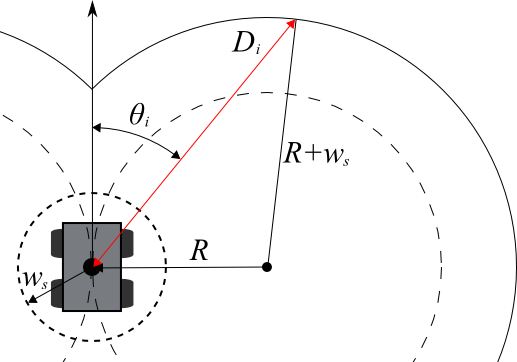
\includegraphics[scale=.4]{figures/DetectionHistogram.png}
\end{figure}
}

\frame{\frametitle{3. Blocked Directions - Masked Histogram}
The masked histogram $M_i = d_i - D_i$ , which shows whethter the steering angle is blocked by obstacles.
\begin{figure}
	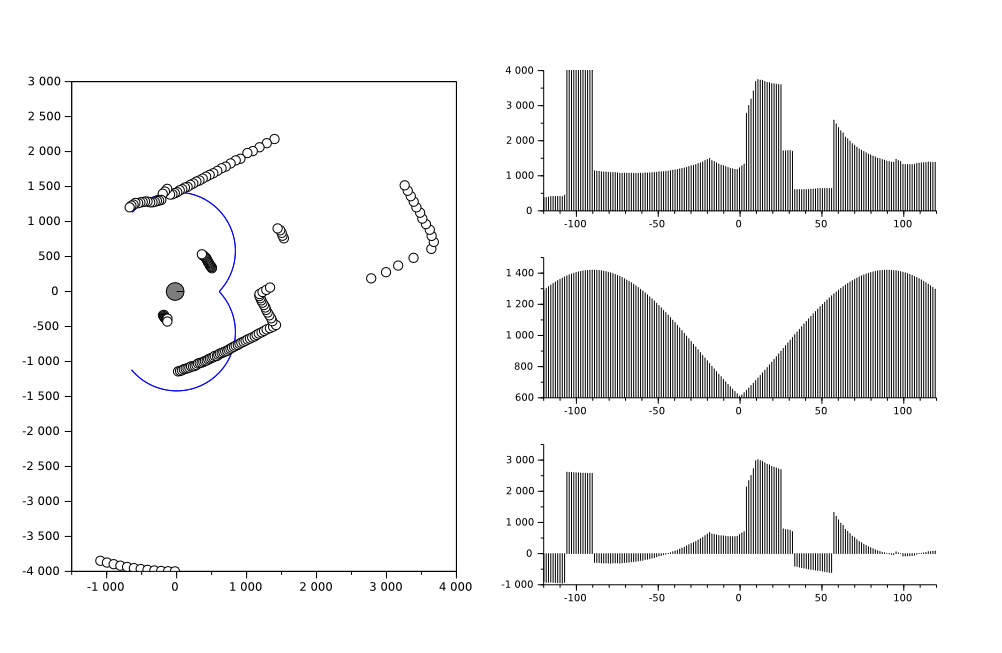
\includegraphics[scale=.35]{figures/MaskedHistogram.png}
\end{figure}
}

\frame{\frametitle{3. Blocked Directions - Determine $\varphi_r$ and $\varphi_l$}
$\varphi_r$ and $\varphi_l$ can be efficiently found by following method: \\
\vspace{0.25cm}
\textrm{1)  Initially set }$\varphi_r = -\pi$\textrm{ and }$\varphi_l = \pi$ \\
\vspace{0.25cm}
\textrm{2) For every }$M_i < 0$\textrm{:} \\
\vspace{0.25cm}
\hspace{0.4cm} \textrm{a) If }$\theta_i < 0$\textrm{ and }$\theta_i > \varphi_r$\textrm{ , set }$\varphi_r$\textrm{ to }$\theta_i$ \\
\vspace{0.25cm}
\hspace{0.4cm} \textrm{a) If }$\theta_i > 0$\textrm{ and }$\theta_i < \varphi_l$\textrm{ , set }$\varphi_l$\textrm{ to }$\theta_i$ \\
}

\frame{\frametitle{4. Selection of Steering Direction - Candidate Direcions}
A set of candidate directions $c_n$ are selected from $\theta_i$ which satisfied:
\[
	\theta_i\in(\varphi_r,\varphi_l) \cap (V_1' \cup V_2' \cup \cdots \cup V_j')
\]
\begin{figure}
	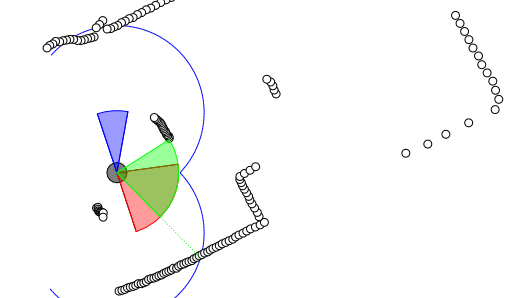
\includegraphics[scale=.5]{figures/CandidateDirections2.png}
\end{figure}
}

\frame{\frametitle{4. Selection of Steering Direction - Cost Function}
Like VFH, VFH$^+$ also uses a cost function to select the preferred direction $c_t$:
\begin{align*}
	G(c_n) &= u_{1} \cdot (|c_n - \varphi_t|) + u_{2} \cdot (c_n) + u_{3} \cdot (|c_n - c_{t-1}|) \\
	\intertext{and}
	c_t &= min \left\{ G(c_n) \right\} \\
	\intertext{where}
	\varphi_t &= \text{Target direction} \\
	c_n &= \text{Candidate direction} \\
	c_{t-1} &= \text{Previously selected directions} \\
\end{align*}
}

\subsection{Algorithm of Speed}
\frame{\frametitle{Algorithm of Speed}
Speed of the robot is controled by the density function $D(d_i)$ of surrounding objects with certain threshold $\tau_{obj}$:
\begin{equation*}
	D(d_i) = \frac{1}{N} \sum_{i=1}^N {H_i}
\end{equation*}
where
\[
	H_i = 
	\begin{cases}
		0	& \textrm{if } d_i \geq \tau_{obj} \\
		1	& \textrm{if } d_i < \tau_{obj} \\
	\end{cases}
\]

With maximum speed $\nu_{max}$ and minimum speed $\nu_{min}$:
\begin{equation*}
	\nu = (\nu_{max} - \nu_{min}) \cdot (1 - D(d_i)) + \nu_{min}
\end{equation*}
}

\subsection{Conclusion}
\frame{\frametitle{Conclusion}
Compare to original VFH method, VFH$^+$ eventually overcomes some defects:
\begin{itemize}
	\item Overcome the primary problem of VFH where steering angle is determined by spaces
	\item Create smooth trajectory by hysteresis threshold
	\item Take robot's geometry and kinematic constraints into account
\end{itemize}
\vspace{0.25cm}
However, it still suffers from some problems:
\begin{itemize}
	\item The geometry of the robot is assumed to be circular
	\item Leads the robot into dead end which can be avoided
\end{itemize}
}


\begin{comment}
\section{General overview of the project}
\subsection{Aims}
\frame{\frametitle{Aims}
The \textbf{general aims} of our research project can be summarised in the following points:
\vspace{0.25cm}
\begin{enumerate}
\item Track \textbf{trends} on the Web by applying Machine Learning methods (track expresses the notions of infer or predict as well)
\vspace{0.25cm}
\item Extend current or invent new \textbf{methodologies} (where and if needed) for accomplishing our primary aim
\vspace{0.25cm}
\item Build \textbf{tools} that apply the experimental/theoretical results in real and large-scale applications (featured research)
\end{enumerate}
}


\subsection{Being more specific}
\frame{\frametitle{Being more specific}
\begin{enumerate}
\item \textbf{Trends} about what? Examples?
      \begin{itemize}
        \item Predict flu rates (\emph{epidemics})
        \item Infer vote intensions (\emph{politics})
        \item Infer traffic/weather conditions (\emph{toy problems})\pause
      \end{itemize}
\vspace{0.25cm}
\item \textbf{Methodologies}?
      \begin{itemize}
        \item Feature extraction/selection
        \item Exploit probabilistic relationships (PGMs)
        \item Regression/classification/ranking scenarios
        \item Active learning\pause
      \end{itemize}
\vspace{0.25cm}
\item \textbf{Applications}?
      \begin{itemize}
        \item Back-end infrastructure for data collection/retrieval/mining
        \item Real time online tools for making and displaying predictions (like the \href{http://geopatterns.enm.bris.ac.uk/epidemics/}{\textbf{Flu detector}})
      \end{itemize}
\end{enumerate}
}

\section{Last 6 months}
\subsection{P1: Tracking the flu pandemic by monitoring the Social Web}
\frame{\frametitle{P1 - Summary (1 of 3)}
{\footnotesize
\begin{tabbing}
Title: \hspace{1.25cm} \= \textbf{Tracking the flu pandemic by monitoring the Social Web}\\
Authors:               \> V. Lampos and N. Cristianini\\
Submitted to:          \> IAPR Cognitive Information Processing 2010 (accepted)
\end{tabbing}
}
\begin{itemize}
\item Twitter and Health Protection Agency data for weeks 26-49, 2009 (on average 160,000 tweets collected per day geolocated in 54 urban centres in the UK)
\item Frequency of \textbf{41 flu related words} (markers) in Twitter corpus had a correlation of $>$\textbf{80\%} with the HPA flu rates in all UK regions
\item Learn a better list of weighted markers \textbf{automatically}:
    \begin{itemize}
    \item Generate a list of candidate markers (1560 words taken from flu related web pages)
    \item Use \textbf{LASSO} for feature selection
    \end{itemize}
\end{itemize}
}

\frame{\frametitle{P1 - Summary (2 of 3)}

\textbf{Validation} schemes:
    \begin{enumerate}
    \item Train on one region, validate regularisation parameter on another, test on the remaining regions (for all possible combinations)

    \begin{table}[!t]
    \tiny
    \renewcommand{\arraystretch}{1}
    \centering
    \begin{tabular}{cccccc}
    \hline
    Train/Validate (regions) & \textbf{A} & \textbf{B}      & \textbf{C} & \textbf{D}       & \textbf{E}     \\\hline
    \textbf{A}     & -          & 0.9594          & 0.9375     & 0.9348           & 0.9297         \\%\hline
    \textbf{B}     & 0.9455     & -               & 0.9476     & 0.9267           & 0.9003         \\%\hline
    \textbf{C}     & 0.9154     & 0.9513          & -          & 0.8188           & 0.908          \\%\hline
    \textbf{D}     & 0.9463     & 0.9459          & 0.9424     & -                & 0.9337         \\%\hline
    \textbf{E}     & 0.8798     & 0.9506          & 0.9455     & 0.8935           & -              \\\hline
    &              &            &\multicolumn{2}{c}{Total Avg.}                   & \textbf{0.9256}\\\cline{4-6}
    \end{tabular}
    \end{table}

    \begin{spacing}{0.5}{
    \textbf{97 selected words}\tiny : lung, unwel, temperatur, like, headach, season, unusu, chronic, child, dai, appetit, stai, symptom, spread, diarrhoea, start, muscl, weaken, immun, feel, liver, plenti, antivir, follow,
    sore, peopl, nation, small, pandem, pregnant, thermomet, bed, loss, heart, mention, condit, ...
    }
    \end{spacing}

    \item Aggregate data from all regions, test on weeks 28 and 41 (2009) and train using the rest of the data set
    \end{enumerate}
}

\frame{\frametitle{P1 - Summary (3 of 3)}
\begin{enumerate}
\item Inferred vs Official flu rate in North England\\
\centering \includegraphics[scale=.5]{figures/Lasso_Inference_regionC_NEng.pdf}

\item Inferred vs Official rates in all regions (aggregated data set)\\
\centering \includegraphics[scale=.5]{figures/Lasso_Inference_Aggregate_IMPROVED.pdf}

\end{enumerate}
}

\subsection{P2: Flu detector - Tracking epidemics on Twitter}
\frame{\frametitle{P2 - Summary}
{\footnotesize
\begin{tabbing}
Title: \hspace{1.25cm} \= \textbf{Flu detector - Tracking epidemics on Twitter}\\
Authors:               \> V. Lampos, T. De Bie, and N. Cristianini\\
Submitted to:          \> ECML PKDD 2010 Demos (under review)
\end{tabbing}
}

\begin{itemize}
\item Extending and making more robust the methodology of P1
\item Larger data sets (bigger time series) and more (2675) \href{http://geopatterns.enm.bris.ac.uk/epidemics/files/candidate_features.txt}{candidate features}
\item Select a list of features (markers) using BoLASSO (bootstrap version of LASSO)
\item Then learn weights of those markers via linear least squares regression
\item Stricter evaluation of the methodology - \href{http://geopatterns.enm.bris.ac.uk/epidemics/twitter-flu-eval.php}{\textbf{Available online}}
\item Put all this into practice and come up with the \href{http://geopatterns.enm.bris.ac.uk/epidemics/}{\textbf{Flu detector}}
\end{itemize}
}

\subsection{Other activities}
\frame{\frametitle{Other activities}
\begin{itemize}
\item Studied/implemented the necessary statistical tools and algorithms (in MATLAB or Java)
\item Extended further the infrastructure for conducting large scale experiments and data retrieval on demand
\item TA for Intro to AI, Data Analysis and Pattern Analysis \& Statistical Learning
\item Attended some of the ISL meetings and seminars
\end{itemize}
}

\section{Next 6 months}
\subsection{General goals \& activities}
\frame{\frametitle{General goals \& activities}
\begin{enumerate}
\item ... (content omitted)
\item ... (content omitted)
\item ... (content omitted)
\item ... (content omitted)
\end{enumerate}
}

\subsection{A more time specific tentative plan}
\frame{\frametitle{A more time specific tentative plan}
\begin{itemize}
\item In \textbf{June}: ... (content omitted)
\item In \textbf{July}: ... (content omitted)
\item In \textbf{August}: ... (content omitted)
\item In \textbf{September - November}: ... (content omitted)
\end{itemize}
}

\section*{}
\frame{
    \begin{center}
        \huge
        This is the last slide.\\ \pause
        \vspace{1cm}
        Any questions?
    \end{center}
}
\end{comment}

%\bibliographystyle{abbrv}
%\bibliography{../../thesis/thesis}
\end{document}
